
% Table is required for multicolumn package with beamer
\documentclass[table]{beamer}

\usepackage{pucv_jz}

\title{Datos Multivariados}
\subtitle{Estadística Computacional}
\author[J.Z.O-2023]{Juan Zamora Osorio\\\url{juan.zamora@pucv.cl}}
\institute[PUCV]{Instituto de Estadística\\Pontificia Universidad Cat\'olica de Valpara\'iso}
\date{\today}


%%%%%%%%xxx
\begin{document}

\frame{\titlepage}

%\begin{frame}
%\frametitle{Contents}
%\tableofcontents
%\end{frame}

% \section{Motivation}

%\begin{frame}
%\frametitle{Contents}
%\tableofcontents[currentsection]
%\end{frame}

\begin{frame}
    \frametitle{Datos bivariados}
    \begin{center}
        \begin{tabular}{c|c|c}
            id Pasajero & Clase & Satisfacción \\
            \hline
            1 & E & 2 \\
            2 & E & 4 \\
            3 & E & 1 \\
            4 & B & 3 \\
            5 & E & 1 \\
            6 & B & 2 \\
            7 & P & 4 \\
            8 & E & 3 \\
            9 & E & 2 \\
            10 & B & 4 \\
            11 & E & 3 \\
            12 & B & 3 \\
            $\vdots$ & $\vdots$ & $\vdots$
        \end{tabular}
    \end{center}
\end{frame}

\begin{frame}
    \frametitle{Datos bivariados categóricos -- tabla de contingencia}
    \begin{center}

\resizebox{10cm}{!}{

        \begin{tabular}{c|c|c}
            id Pasajero & Clase & Satisfacción \\
            \hline
            1 & E & 2 \\
            2 & E & 4 \\
            3 & E & 1 \\
            4 & B & 3 \\
            5 & E & 1 \\
            6 & B & 2 \\
            7 & P & 4 \\
            8 & E & 3 \\
            9 & E & 2 \\
            10 & B & 4 \\
            11 & E & 3 \\
            12 & B & 3 \\
            $\vdots$ & $\vdots$ & $\vdots$
        \end{tabular}

        \begin{tabular}{c|c|cccc|c}
            & & \multicolumn{4}{c|}{Satisfacción} & Total \\
            \hline
            & & 1 & 2 & 3 & 4 & \\
            \hline
            & E & 2 & 2 & 2 & 1 & 7 \\
            Clase & B & 0 & 1 & 2 & 1 & 4 \\
            & P & 0 & 0 & 0 & 1 & 1 \\
            \hline
            Total & & 2 & 3 & 4 & 3 & 12
        \end{tabular}

}

    \end{center}
\end{frame}

\begin{frame}
    \frametitle{Datos bivariados categóricos -- tabla de contingencia}
    \begin{center}
        \begin{tabular}{c|c|cccc|c}
            & & \multicolumn{4}{c|}{Satisfacción} & Total \\
            \hline
            & & 1 & 2 & 3 & 4 & \\
            \hline
            & E & 10 & 33 & 15 & 4 & 62 \\
            Clase & B & 0 & 3 & 20 & 2 & 25 \\
            & P & 0 & 0 & 5 & 8 & 13 \\
            \hline
            Total & & 10 & 36 & 40 & 14 & 100
        \end{tabular}
    \end{center}
    \begin{block}{Clases bivariadas}
        \begin{itemize}
            \item $\parens{\text{E} , 1}$, $\parens{\text{E} , 2}$, $\parens{\text{E} , 3}$, $\parens{\text{E} , 4}$, $\parens{\text{B} , 2}$, $\parens{\text{B} , 3}$, $\parens{\text{B} , 4}$, $\parens{\text{P}, 3}$, $\parens{\text{P} , 4}$.
            \item ¡Pueden ser muchas!
        \end{itemize}
    \end{block}
\end{frame}

\begin{frame}
    \frametitle{Datos bivariados categóricos -- tabla de contingencia}
    \begin{center}
        \begin{tabular}{c|c|ccccc|c}
            & & \multicolumn{5}{c|}{$Y$} & Total \\
            \hline
            & & $y_{1}$ & $\cdots$ & $y_{j}$ & $\cdots$ & $y_{J}$ & \\
            \hline
            & $x_{1}$ & $n_{11}$ & $\cdots$ & $n_{1j}$ & $\cdots$ & $n_{1J}$ & $n_{1 \cdot}$ \\
             & $\vdots$ & $\vdots$ & $\ddots$ & $\vdots$ & $\ddots$ & $\vdots$ & $\vdots$ \\
            $X$ & $x_{k}$ & $n_{k1}$ & $\cdots$ & $n_{kj}$ & $\cdots$ & $n_{kJ}$ & $n_{k \cdot}$ \\
             & $\vdots$ & $\vdots$ & $\ddots$ & $\vdots$ & $\ddots$ & $\vdots$ & $\vdots$ \\
            & $x_{K}$ & $n_{K1}$ & $\cdots$ & $n_{Kj}$ & $\cdots$ & $n_{KJ}$ & $n_{K \cdot}$ \\
            \hline
            Total & & $n_{\cdot 1}$ & $\cdots$ & $n_{\cdot j}$ & $\cdots$ & $n_{\cdot J}$ & $n$ \\
        \end{tabular}
    \end{center}
    \begin{block}{Frecuencias absolutas marginales}
        \begin{equation*}
            n = \sum_{k = 1}^{K} n_{k \cdot} = \sum_{j = 1}^{j} n_{\cdot j} = \sum_{k = 1}^{K} \sum_{j = 1}^{J} n_{k j} .
        \end{equation*}
    \end{block}
\end{frame}

\begin{frame}
    \frametitle{Datos bivariados categóricos -- tabla de contingencia}
    \begin{center}
        \begin{tabular}{c|c|ccccc|c}
            & & \multicolumn{5}{c|}{$Y$} & Total \\
            \hline
            & & $y_{1}$ & $\cdots$ & $y_{j}$ & $\cdots$ & $y_{J}$ & \\
            \hline
            & $x_{1}$ & $f_{11}$ & $\cdots$ & $f_{1j}$ & $\cdots$ & $f_{1J}$ & $f_{1 \cdot}$ \\
             & $\vdots$ & $\vdots$ & $\ddots$ & $\vdots$ & $\ddots$ & $\vdots$ & $\vdots$ \\
            $X$ & $x_{k}$ & $f_{k1}$ & $\cdots$ & $f_{kj}$ & $\cdots$ & $f_{kJ}$ & $f_{k \cdot}$ \\
             & $\vdots$ & $\vdots$ & $\ddots$ & $\vdots$ & $\ddots$ & $\vdots$ & $\vdots$ \\
            & $x_{K}$ & $f_{K1}$ & $\cdots$ & $f_{Kj}$ & $\cdots$ & $f_{KJ}$ & $f_{K \cdot}$ \\
            \hline
            Total & & $f_{\cdot 1}$ & $\cdots$ & $f_{\cdot j}$ & $\cdots$ & $f_{\cdot J}$ & $1$ \\
        \end{tabular}
    \end{center}
    \begin{block}{Frecuencias relativas marginales}
        \begin{equation*}
            1 = \sum_{k = 1}^{K} f_{k \cdot} = \sum_{j = 1}^{j} f_{\cdot j} = \sum_{k = 1}^{K} \sum_{j = 1}^{J} f_{k j} .
        \end{equation*}
    \end{block}
\end{frame}

\begin{frame}
    \frametitle{Datos bivariados categóricos -- frecuencias condicionales}
    \begin{center}
        \begin{tabular}{c|c|ccccc|c}
            & & \multicolumn{5}{c|}{$Y$} & Total \\
            \hline
            & & $y_{1}$ & $\cdots$ & $y_{j}$ & $\cdots$ & $y_{J}$ & \\
            \hline
            & $x_{1}$ & $f_{11}$ & $\cdots$ & $f_{1j}$ & $\cdots$ & $f_{1J}$ & $f_{1 \cdot}$ \\
             & $\vdots$ & $\vdots$ & $\ddots$ & $\vdots$ & $\ddots$ & $\vdots$ & $\vdots$ \\
            $X$ & $x_{k}$ & $f_{k1}$ & $\cdots$ & $f_{kj}$ & $\cdots$ & $f_{kJ}$ & $f_{k \cdot}$ \\
             & $\vdots$ & $\vdots$ & $\ddots$ & $\vdots$ & $\ddots$ & $\vdots$ & $\vdots$ \\
            & $x_{K}$ & $f_{K1}$ & $\cdots$ & $f_{Kj}$ & $\cdots$ & $f_{KJ}$ & $f_{K \cdot}$ \\
            \hline
            Total & & $f_{\cdot 1}$ & $\cdots$ & $f_{\cdot j}$ & $\cdots$ & $f_{\cdot J}$ & $1$ \\
        \end{tabular}
    \end{center}
    \begin{block}{Frecuencias condicionales}
            \begin{equation*}
                f_{k \mid j} = \frac{f_{k j}}{f_{\cdot j}} = \frac{n_{k j}}{n_{\cdot j}} ,
            \end{equation*}
            \begin{equation*}
                f_{j \mid k} = \frac{f_{k j}}{f_{k \cdot}} = \frac{n_{k j}}{n_{k \cdot}} .
            \end{equation*}
    \end{block}
\end{frame}

\begin{frame}
    \frametitle{Ejemplo -- satisfacción de vuelos}
    \begin{center}
        \begin{tabular}{c|c|cccc|c}
            & & \multicolumn{4}{c|}{Satisfacción} & Total \\
            \hline
            & & 1 & 2 & 3 & 4 & \\
            \hline
            & E & 10 & 33 & 15 & 4 & 62 \\
            Clase & B & 0 & 3 & 20 & 2 & 25 \\
            & P & 0 & 0 & 5 & 8 & 13 \\
            \hline
            Total & & 10 & 36 & 40 & 14 & 100
        \end{tabular}
        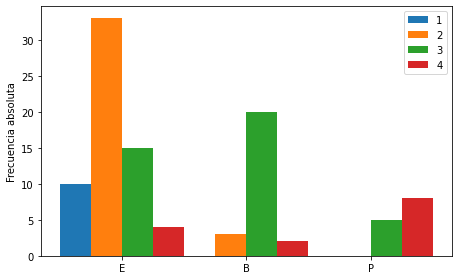
\includegraphics[width=0.49\textwidth]{barras_por_clase_1}
        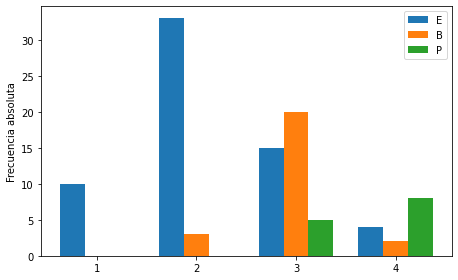
\includegraphics[width=0.49\textwidth]{barras_por_clase_2}
    \end{center}
\end{frame}

\begin{frame}
    \frametitle{Ejemplo -- satisfacción de vuelos}
    \begin{center}
        \begin{tabular}{c|c|cccc|c}
            & & \multicolumn{4}{c|}{Satisfacción} & Total \\
            \hline
            & & 1 & 2 & 3 & 4 & \\
            \hline
            & E & 10 & 33 & 15 & 4 & 62 \\
            Clase & B & 0 & 3 & 20 & 2 & 25 \\
            & P & 0 & 0 & 5 & 8 & 13 \\
            \hline
            Total & & 10 & 36 & 40 & 14 & 100
        \end{tabular}
        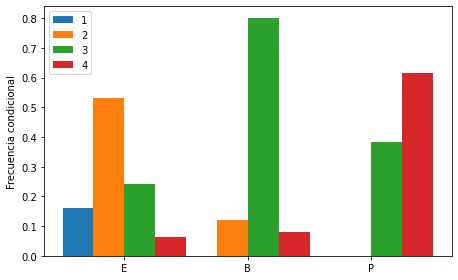
\includegraphics[width=0.49\textwidth]{barras_condicionales_1}
        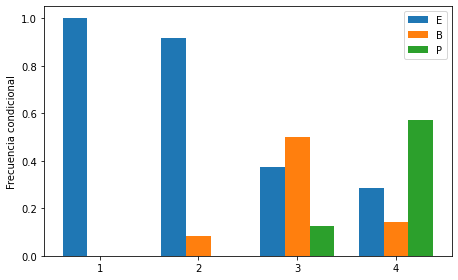
\includegraphics[width=0.49\textwidth]{barras_condicionales_2}
    \end{center}
\end{frame}

\begin{frame}
    \frametitle{Ejemplo -- satisfacción de vuelos}
    \begin{center}
        \begin{tabular}{c|c|cccc|c}
            & & \multicolumn{4}{c|}{Satisfacción} & Total \\
            \hline
            & & 1 & 2 & 3 & 4 & \\
            \hline
            & E & 10 & 33 & 15 & 4 & 62 \\
            Clase & B & 0 & 3 & 20 & 2 & 25 \\
            & P & 0 & 0 & 5 & 8 & 13 \\
            \hline
            Total & & 10 & 36 & 40 & 14 & 100
        \end{tabular}
        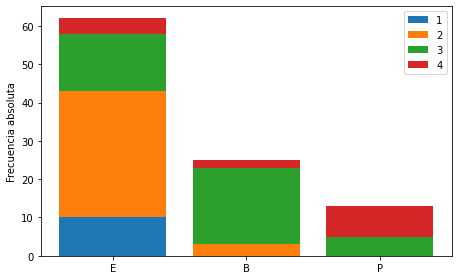
\includegraphics[width=0.49\textwidth]{barras_stacked_1}
        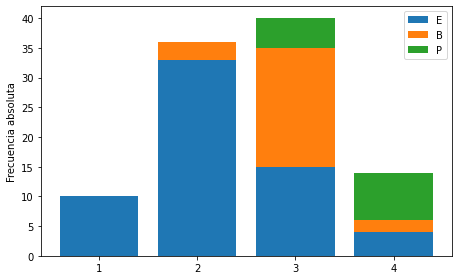
\includegraphics[width=0.49\textwidth]{barras_stacked_2}
    \end{center}
\end{frame}

\begin{frame}
    \frametitle{Ejemplo -- satisfacción de vuelos}
    \begin{center}
        \begin{tabular}{c|c|cccc|c}
            & & \multicolumn{4}{c|}{Satisfacción} & Total \\
            \hline
            & & 1 & 2 & 3 & 4 & \\
            \hline
            & E & 10 & 33 & 15 & 4 & 62 \\
            Clase & B & 0 & 3 & 20 & 2 & 25 \\
            & P & 0 & 0 & 5 & 8 & 13 \\
            \hline
            Total & & 10 & 36 & 40 & 14 & 100
        \end{tabular}
        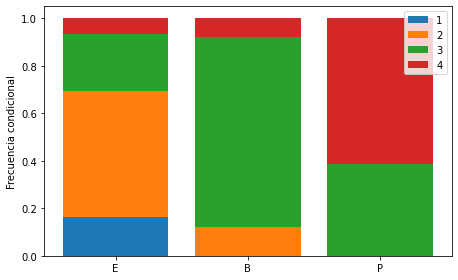
\includegraphics[width=0.49\textwidth]{barras_condicionales_stacked_1}
        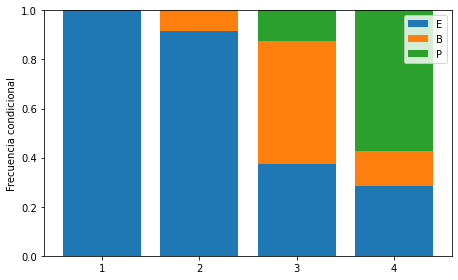
\includegraphics[width=0.49\textwidth]{barras_condicionales_stacked_2}
    \end{center}
\end{frame}

\begin{frame}
    \frametitle{Independencia}
    \begin{center}
        \begin{tabular}{c|c|cccc|c}
            & & \multicolumn{4}{c|}{Satisfacción} & Total \\
            \hline
            & & 1 & 2 & 3 & 4 & \\
            \hline
            & E & 10 & 33 & 15 & 4 & 62 \\
            Clase & B & 0 & 3 & 20 & 2 & 25 \\
            & P & 0 & 0 & 5 & 8 & 13 \\
            \hline
            Total & & 10 & 36 & 40 & 14 & 100
        \end{tabular}
    \end{center}
    \begin{block}{Se busca}
        \begin{itemize}
            \item $f_{k \mid j} = f_{k \cdot}$ y $f_{j \mid k} = f_{\cdot j}$.
        \end{itemize}
    \end{block}
    \begin{block}{Luego}
        \begin{equation*}
            f_{k j} = f_{k \cdot} f_{\cdot j} .
        \end{equation*}
        \begin{itemize}
            \item Esperamos frecuencia absoluta $n_{k j} = n f_{k j} = n f_{k \cdot} f_{\cdot j} = n \frac{n_{k \cdot}}{n} \frac{n_{\cdot j}}{n} = \frac{n_{k \cdot} n_{\cdot j}}{n}$.
        \end{itemize}
    \end{block}
\end{frame}

\begin{frame}
    \frametitle{Independencia}
    \begin{center}
        \begin{tabular}{c|c|cccc|c}
            & & \multicolumn{4}{c|}{Satisfacción} & Total \\
            \hline
            & & 1 & 2 & 3 & 4 & \\
            \hline
            & E & 10 & 33 & 15 & 4 & 62 \\
            Clase & B & 0 & 3 & 20 & 2 & 25 \\
            & P & 0 & 0 & 5 & 8 & 13 \\
            \hline
            Total & & 10 & 36 & 40 & 14 & 100
        \end{tabular}
        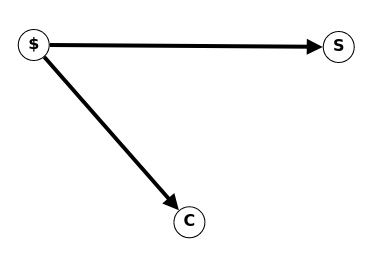
\includegraphics[width=0.47\textwidth]{grafo_dependencia}
    \end{center}
\end{frame}

\begin{frame}
    \frametitle{Datos bivariados continuos}
    \begin{center}
        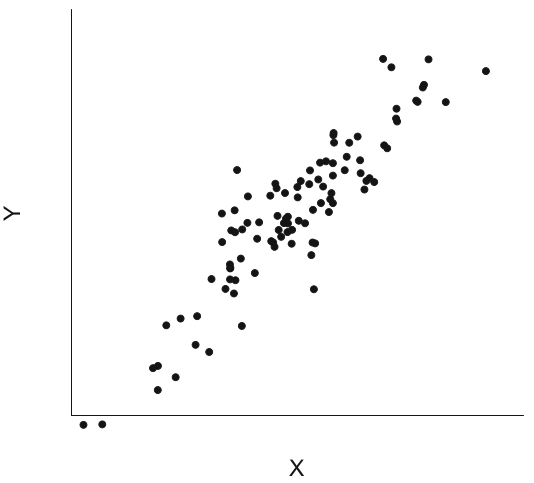
\includegraphics[width=0.35\textwidth]{scatter_1}
        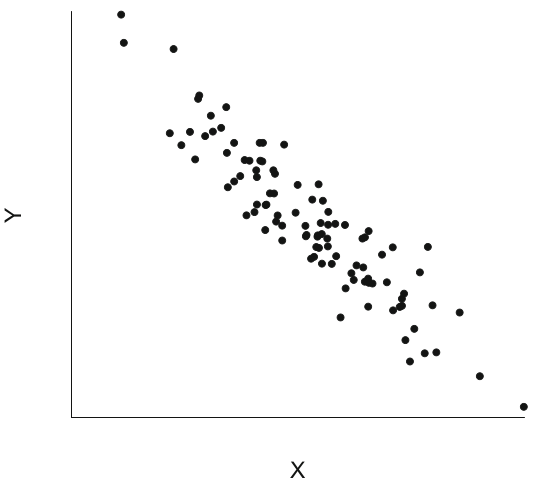
\includegraphics[width=0.35\textwidth]{scatter_2}
        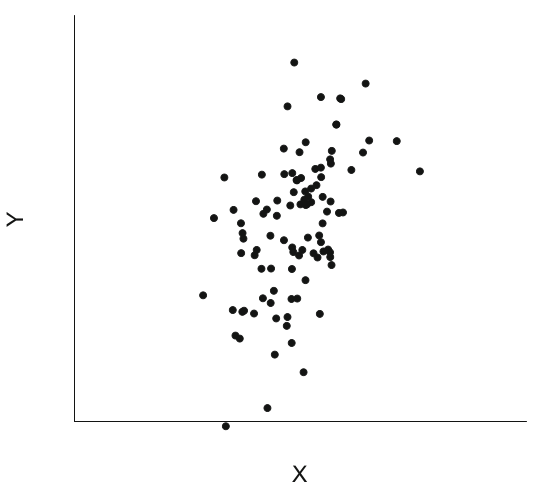
\includegraphics[width=0.35\textwidth]{scatter_3}
        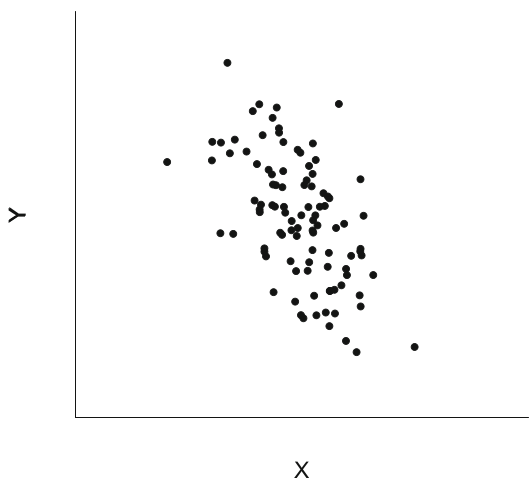
\includegraphics[width=0.35\textwidth]{scatter_4}
    \end{center}
\end{frame}

\begin{frame}
    \frametitle{Gráficos de dispersión (\emph{scatter})}
    \begin{center}
        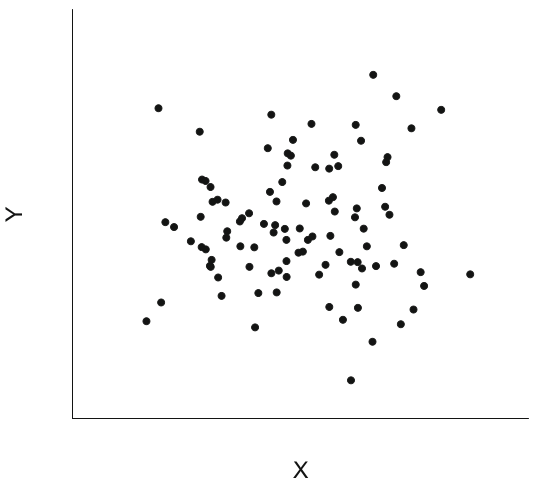
\includegraphics[width=0.35\textwidth]{scatter_5}
        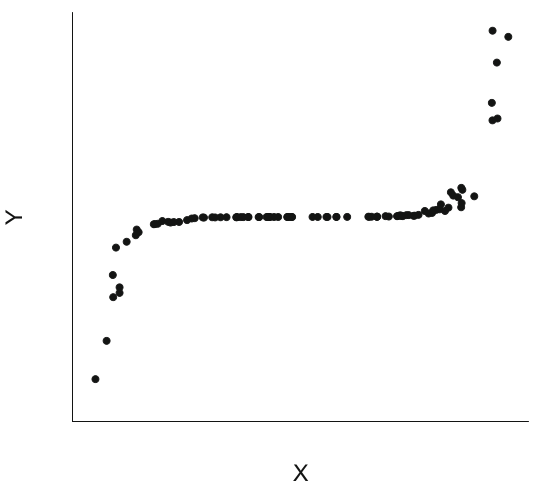
\includegraphics[width=0.35\textwidth]{scatter_6}
    \end{center}
\end{frame}

\begin{frame}
    \frametitle{Gráficos de dispersión (\emph{scatter})}
    \begin{center}
        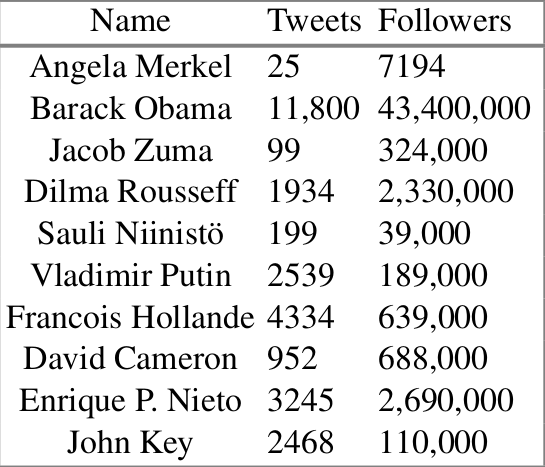
\includegraphics[width=0.4\textwidth]{scatter_datos_ejemplo}
        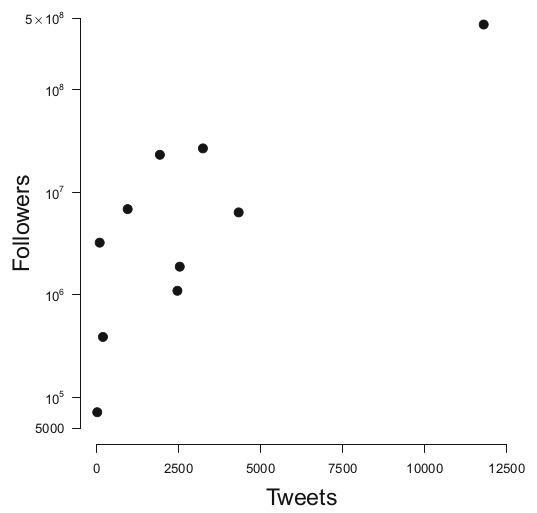
\includegraphics[width=0.49\textwidth]{scatter_log_ejemplo}
    \end{center}
\end{frame}

\begin{frame}
    \frametitle{Gráficos de dispersión (\emph{scatter})}
    \begin{center}
        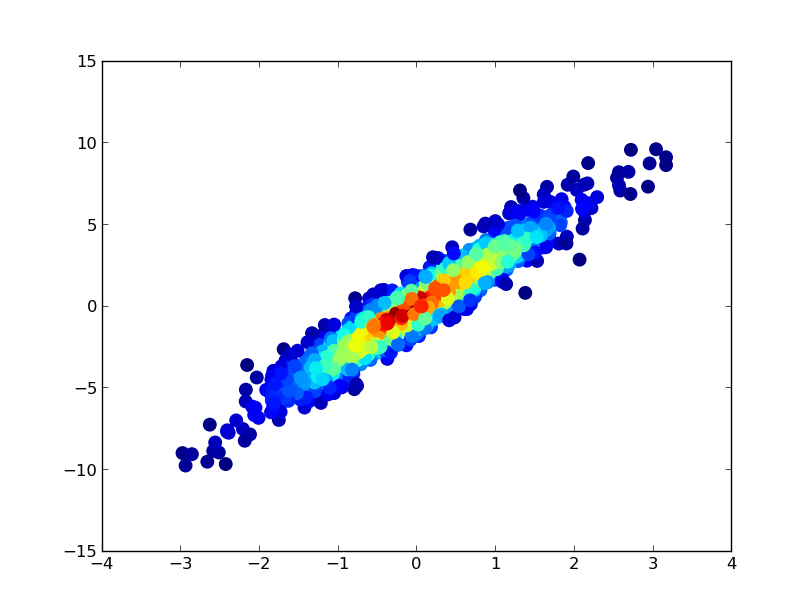
\includegraphics[width=0.49\textwidth]{scatter_color_1}
        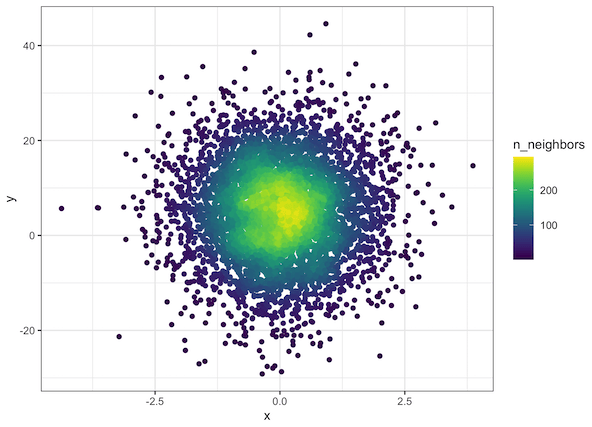
\includegraphics[width=0.49\textwidth]{scatter_color_2}
    \end{center}
\end{frame}

\begin{frame}
    \frametitle{Gráficos de dispersión (\emph{scatter})}
    \begin{center}
        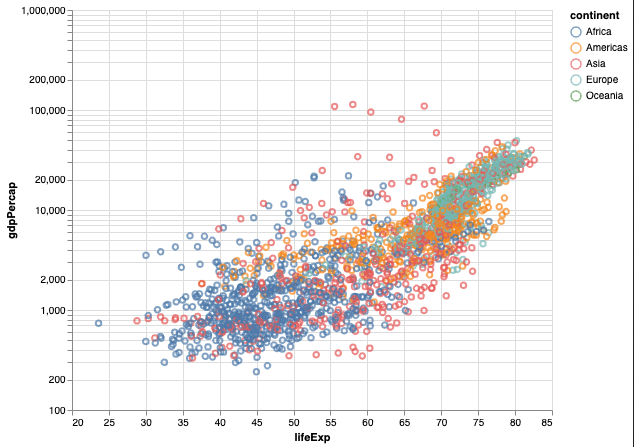
\includegraphics[width=0.49\textwidth]{scatter_avanzado_1}
        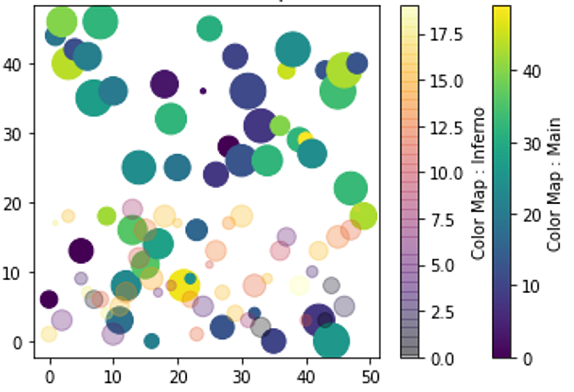
\includegraphics[width=0.49\textwidth]{scatter_avanzado_2}
    \end{center}
\end{frame}

\begin{frame}
    \frametitle{Mapas de calor}
    \begin{center}
        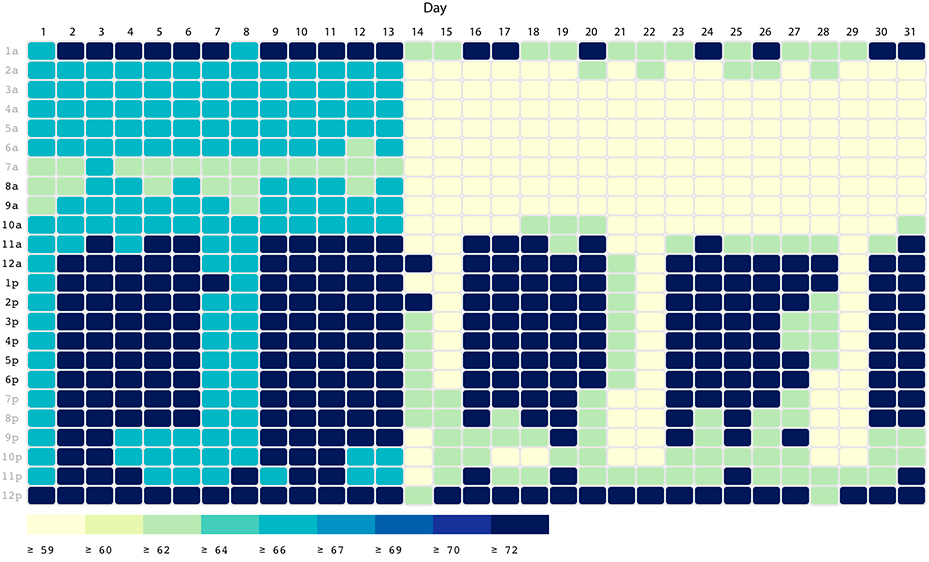
\includegraphics[width=\textwidth]{mapacalor_ejemplo_ameba2}
    \end{center}
\end{frame}

\begin{frame}
    \frametitle{Mapas de calor}
    \begin{center}
        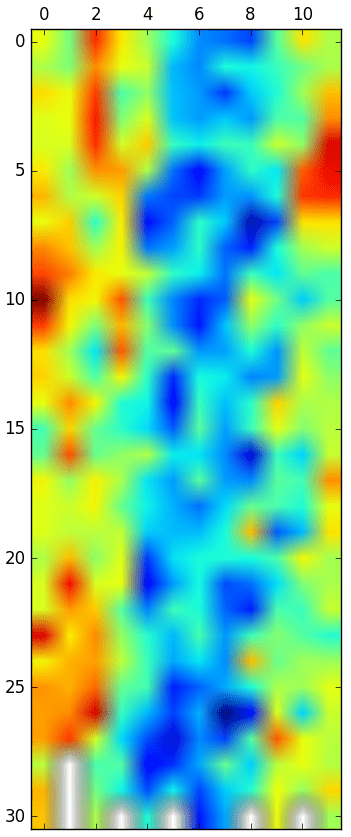
\includegraphics[angle=90, width=0.8\textwidth]{heat_map}
    \end{center}
\end{frame}

\iffalse
\begin{frame}
    \frametitle{Mapas de calor}
    \begin{center}
        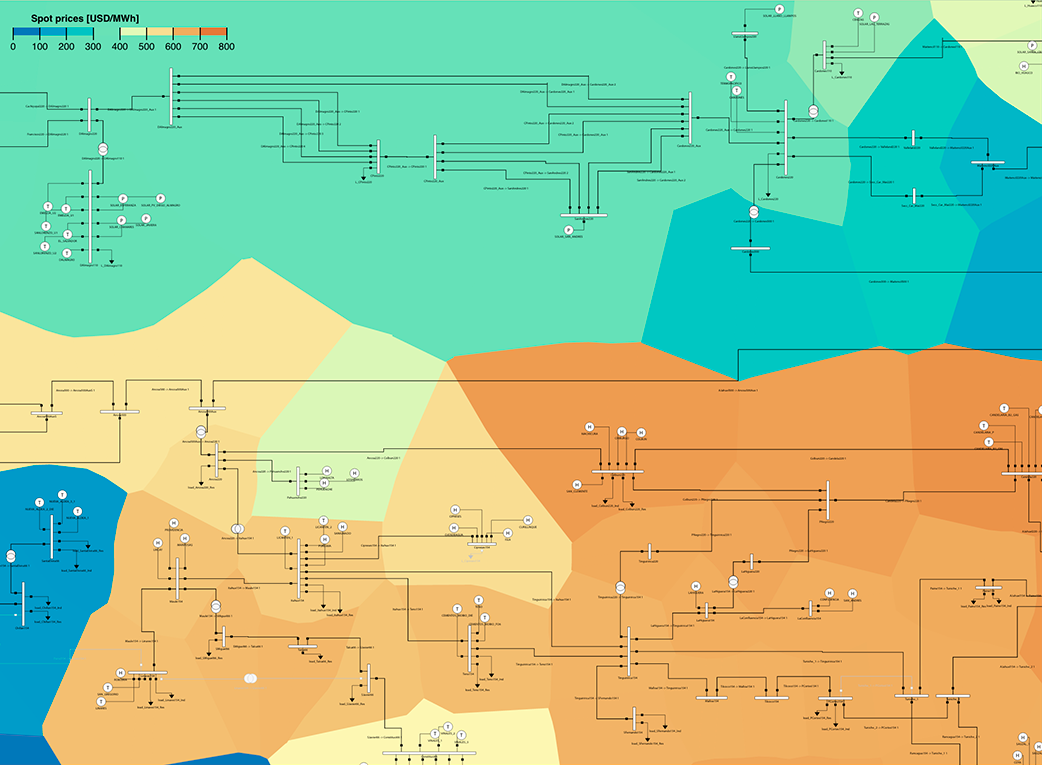
\includegraphics[width=0.8\textwidth]{heatmap_ameba}
    \end{center}
\end{frame}
\fi

\begin{frame}
    \frametitle{Mapas de calor -- contorno}
    \begin{center}
        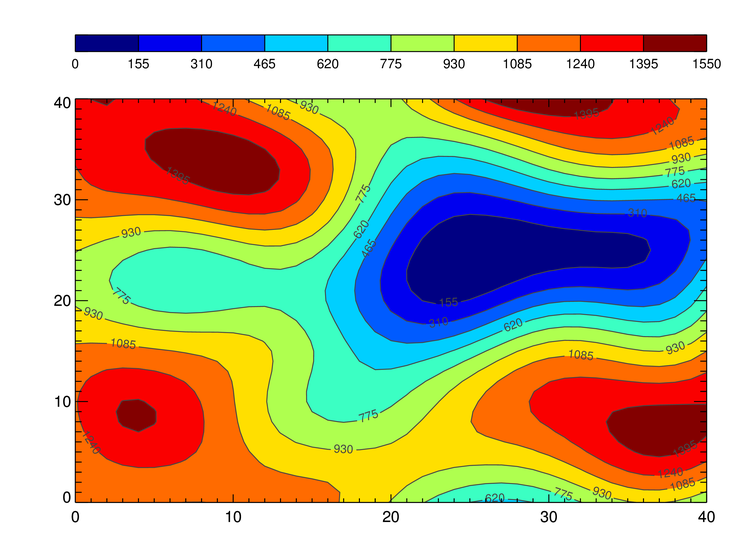
\includegraphics[width=0.8\textwidth]{heat_map_contour}
    \end{center}
\end{frame}

\iffalse
\begin{frame}
    \frametitle{Mapas de calor -- ¡cuidado!}
    \begin{center}
        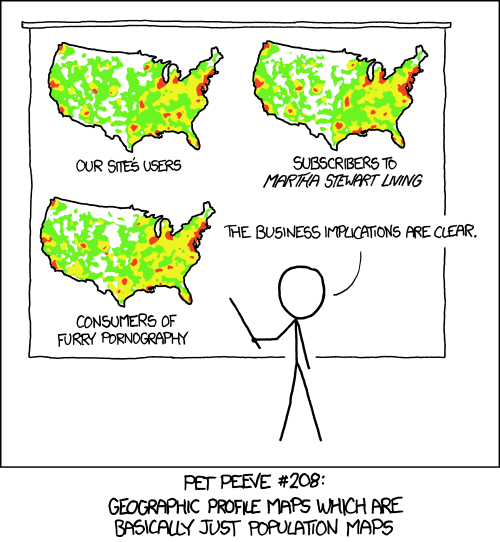
\includegraphics[width=0.6\textwidth]{heatmap}
    \end{center}
\end{frame}
\fi

\begin{frame}
    \frametitle{Datos multivariados}
    \begin{center}
        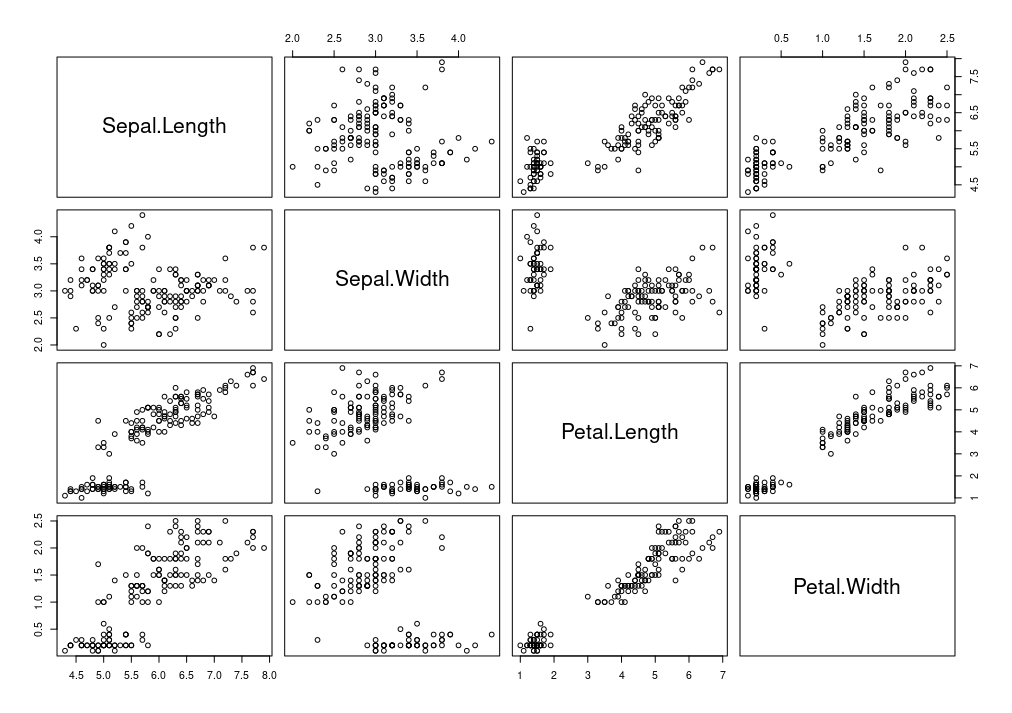
\includegraphics[width=0.8\textwidth]{scatter_tipico}
    \end{center}
\end{frame}

\begin{frame}
    \frametitle{Correlación}
    \begin{block}{Covarianza}
        \begin{equation*}
            \cov{x , y} = \frac{1}{n} \sum_{i = 1}^{n} \parens{x_{i} - \bar{x}} \parens{y_{i} - \bar{y}} .
        \end{equation*}
        \begin{itemize}
            \item Indica dependencia \emph{lineal}.
            \item Notar $\cov{x , x} = s_{x}^{2}$.
        \end{itemize}
    \end{block}
    \begin{block}{Correlación}
        \begin{equation*}
            r_{x y} = \frac{\cov{x , y}}{s_{x} s_{y}} .
        \end{equation*}
        \begin{itemize}
            \item Indica dependencia \emph{lineal}.
            \item Se puede mostrar que $-1 \leq r_{x y} \leq 1$.
        \end{itemize}
    \end{block}
\end{frame}

\begin{frame}
    \frametitle{Correlación}
    \begin{center}
        \begin{tabular}{ccc}
            $r_{x y} = 0.91$ &
            $r_{x y} = -0.92$ &
            $r_{x y} = 0.50$ \\
            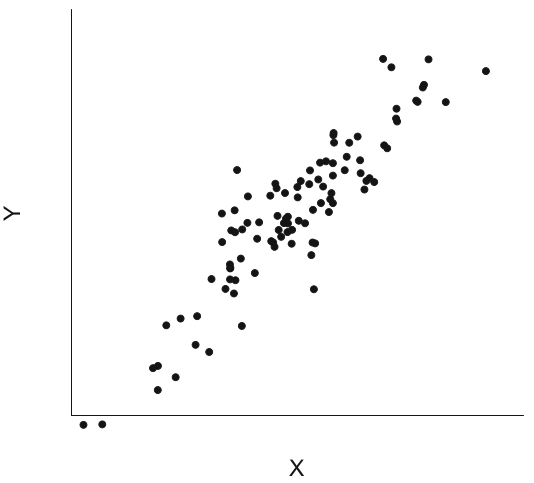
\includegraphics[width=0.3\textwidth]{scatter_1} &
            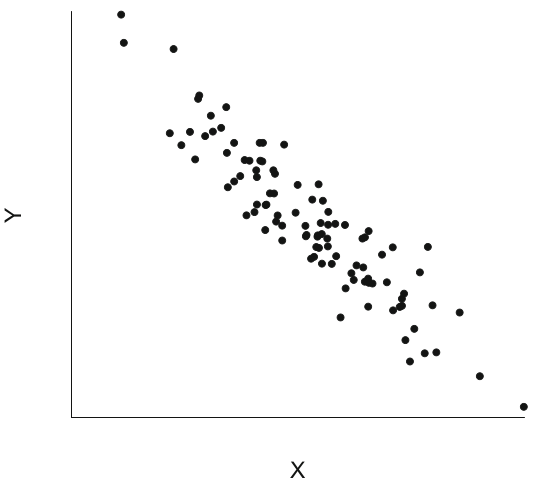
\includegraphics[width=0.3\textwidth]{scatter_2} &
            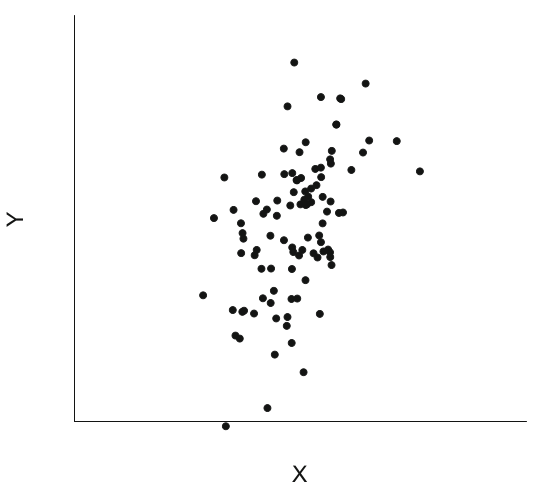
\includegraphics[width=0.3\textwidth]{scatter_3} \\
            $r_{x y} = -0.56$ &
            $r_{x y} = 0.03$ &
            $r_{x y} = 0.64$ \\
            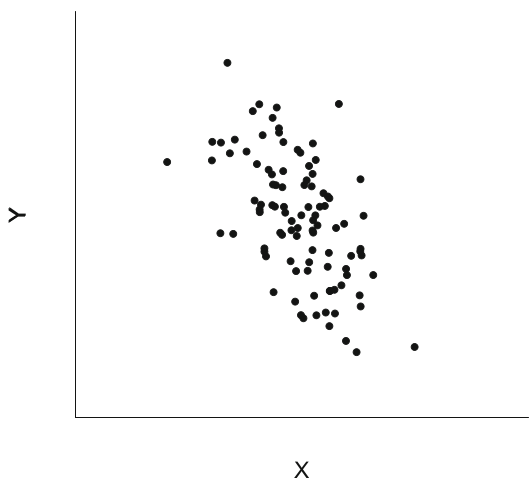
\includegraphics[width=0.3\textwidth]{scatter_4} &
            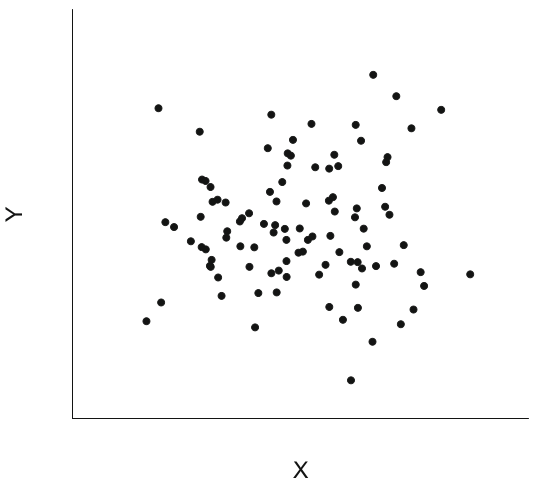
\includegraphics[width=0.3\textwidth]{scatter_5} &
            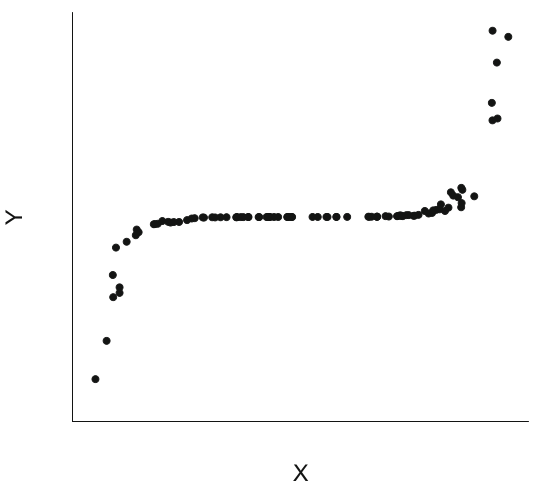
\includegraphics[width=0.3\textwidth]{scatter_6}
        \end{tabular}
    \end{center}
\end{frame}

\begin{frame}
    \frametitle{Matriz de varianzas y covarianzas}
    \begin{equation*}
        \mathbf{S} =
        \begin{bmatrix}
            \cov{x^{1} , x^{1}} & \cdots & \cov{x^{1} , x^{j}} & \cdots & \cov{x^{1} , x^{J}} \\
            \vdots & \ddots & \vdots & \ddots & \vdots \\
            \cov{x^{j} , x^{1}} & \cdots & \cov{x^{j} , x^{j}} & \cdots & \cov{x^{j} , x^{J}} \\
            \vdots & \ddots & \vdots & \ddots & \vdots \\
            \cov{x^{J} , x^{1}} & \cdots & \cov{x^{J} , x^{j}} & \cdots & \cov{x^{J} , x^{J}} \\
        \end{bmatrix}
    \end{equation*}
    \begin{block}{Propiedades}
        \begin{itemize}
            \item Diagonal contiene las varianzas.
            \item Simétrica: $\mathbf{S} = \mathbf{S}^{T}$.
            \item Semidefinida positiva:
                \begin{itemize}
                    \item $\forall a \in \reals^{J} , a^{T} \mathbf{S} a \geq 0$.
                    \item Valores propios son todos no negativos.
                \end{itemize}
        \end{itemize}
    \end{block}
\end{frame}

\begin{frame}
    \frametitle{Matriz de varianzas y covarianzas}
    \begin{block}{Matriz de datos}
        \begin{equation*}
            \mathbf{X} =
            \begin{bmatrix}
                x^{1}_{1} & \cdots & x^{j}_{1} & \cdots & x^{J}_{1} \\
                \vdots & \ddots & \vdots & \ddots & \vdots \\
                x^{1}_{i} & \cdots & x^{j}_{i} & \cdots & x^{J}_{i} \\
                \vdots & \ddots & \vdots & \ddots & \vdots \\
                x^{1}_{n} & \cdots & x^{j}_{n} & \cdots & x^{J}_{n} \\
            \end{bmatrix}
            =
            \begin{bmatrix}
                \mathbf{x}_{1}^{T} \\
                \vdots \\
                \mathbf{x}_{i}^{T} \\
                \vdots \\
                \mathbf{x}_{n}^{T}
            \end{bmatrix}
        \end{equation*}
    \end{block}
    \begin{block}{Construcción}
        \begin{equation*}
            \bar{\mathbf{x}} = \frac{1}{n} \sum_{i = 1}^{n} \mathbf{x}_{i} ,
        \end{equation*}
        \begin{equation*}
            \mathbf{S} = \frac{1}{n} \sum_{i = 1}^{n} \parens{\mathbf{x}_{i} - \bar{\mathbf{x}}} \parens{\mathbf{x}_{i} - \bar{\mathbf{x}}}^{T} .
        \end{equation*}
    \end{block}
\end{frame}

\begin{frame}
    \frametitle{Matriz de correlación}
    \begin{equation*}
        \mathbf{R} =
        \begin{bmatrix}
            1 & \cdots & r_{1 j} & \cdots & r_{1 J} \\
            \vdots & \ddots & \vdots & \ddots & \vdots \\
            r_{j 1} & \cdots & 1 & \cdots & r_{j J} \\
            \vdots & \ddots & \vdots & \ddots & \vdots \\
            r_{J 1} & \cdots & r_{J j} & \cdots & 1 \\
        \end{bmatrix}
    \end{equation*}
    \begin{block}{Propiedades}
        \begin{itemize}
            \item No es igual a la matriz de varianzas y covarianzas escalada.
            \item Se puede construir como $\mathbf{S}$ estandarizando los atributos primero.
        \end{itemize}
    \end{block}
\end{frame}

\begin{frame}
    \frametitle{Matriz de correlación}
    \begin{center}
        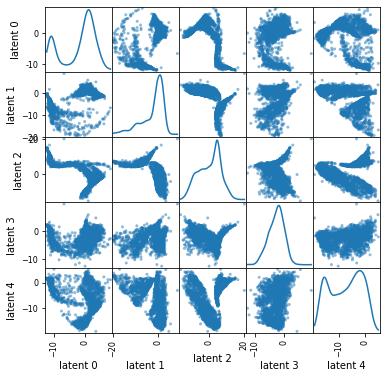
\includegraphics[width=0.49\textwidth]{scatter_small}
        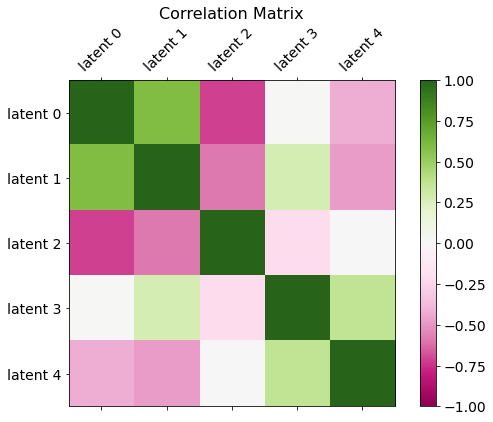
\includegraphics[width=0.49\textwidth]{corr_small}
    \end{center}
\end{frame}

\begin{frame}
    \frametitle{Matriz de correlación}
    \begin{center}
        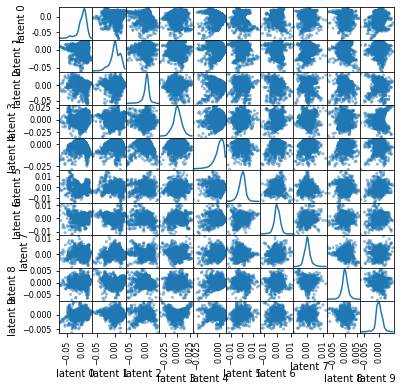
\includegraphics[width=0.49\textwidth]{scatter_big}
        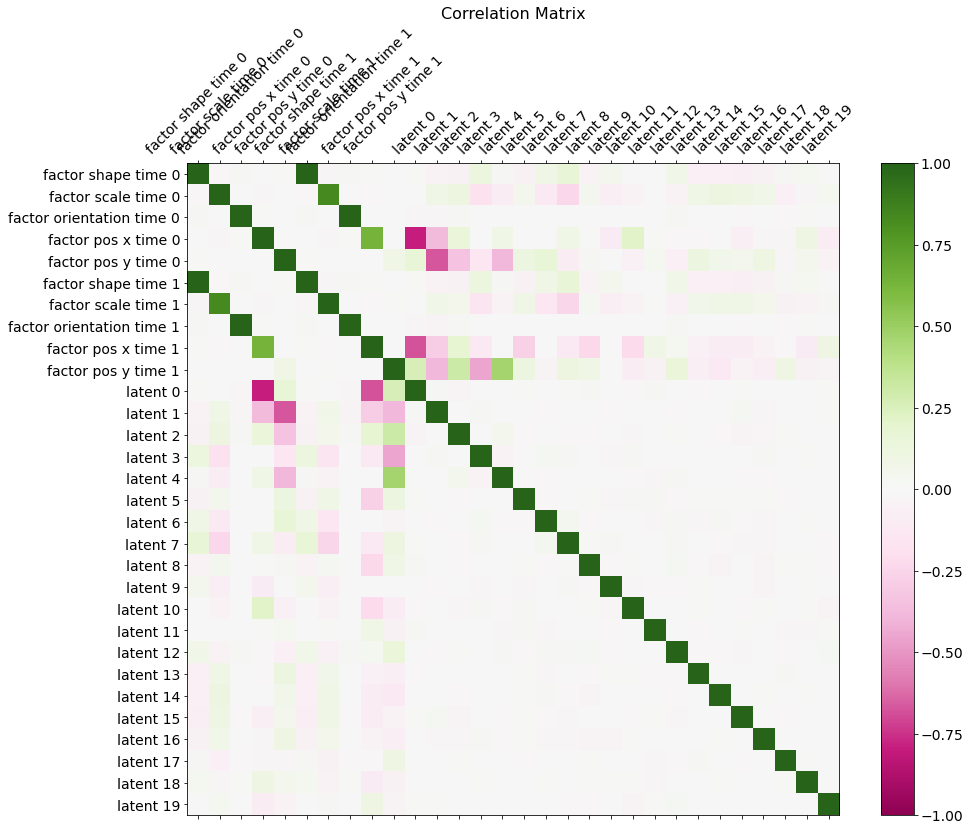
\includegraphics[width=0.49\textwidth]{corr_big}
    \end{center}
\end{frame}

\begin{frame}
    \frametitle{Matrices de correlación y de varianzas y covarianzas}
    \begin{center}
        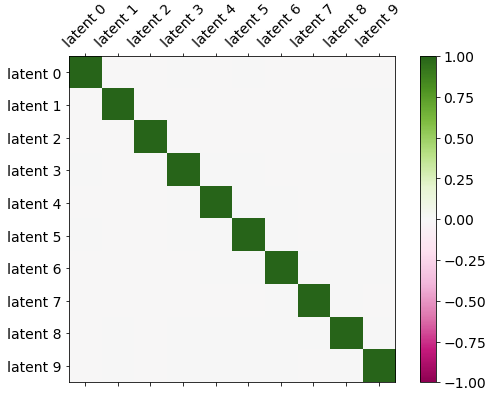
\includegraphics[width=0.49\textwidth]{corr_diagonal}
        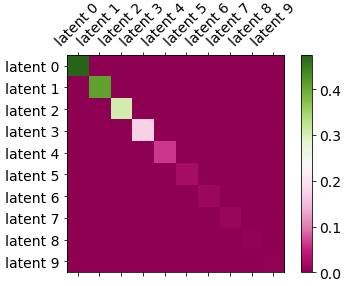
\includegraphics[width=0.49\textwidth]{covar_diagonal}
    \end{center}
\end{frame}

\iffalse
\begin{frame}[allowframebreaks, noframenumbering]
\frametitle<presentation>{References}
\printbibliography
%\bibliographystyle{apalike}
\end{frame}
\fi

\end{document}
